\documentclass[Rapport/Rapport_main.tex]{subfiles}
\begin{document}
\subsection{Systemarkitektur}
Indledningsvis beskrives den overordnede arkitektur for hardware og software for hele systemet. Der kan i figur \ref{fig:rap_systemarkitektur} ses et deployment view, der viser software allokeringer for de overordnede blokke. I den følgende arkitektur benævnes den tidligere benævnte systemcontroller som RPi.
\begin{figure}[H]
    \centering
    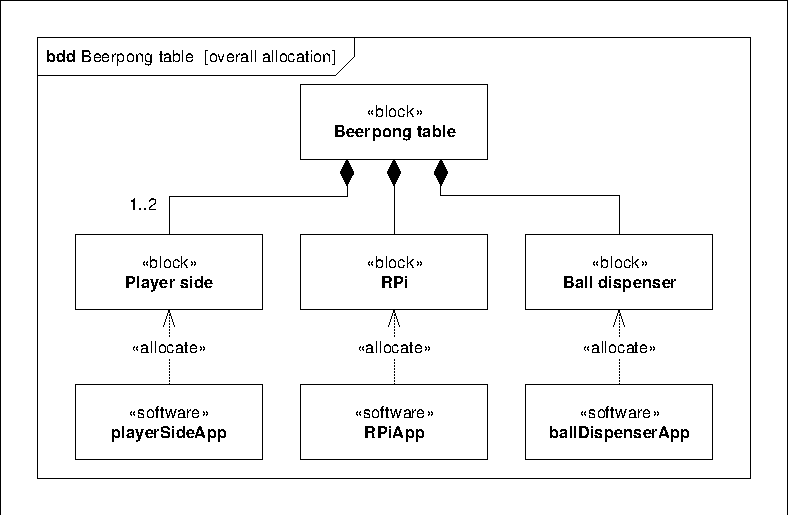
\includegraphics[width=1\textwidth,trim={0.24in 0.24in 0.24in 0.24in},clip, page=1]{Arkitektur/graphics/BDD_og_IBD.pdf}
    \caption{Overordnet blok definitionsdiagram for systemet med software allokeringer. Diagrammet indeholder kun blokke der indeholder CPU'er. Her ses blokkene Playerside, RPi og Balldispenser. Blokkene er udledt i afsnit \fullref{sec:rapport_analyse}.}
    \label{fig:rap_systemarkitektur}
\end{figure}
\textbf{Playerside} blokken kan beskrives, som den blok der håndterer kopperne i enderne på bordet, og som registrerer \textit{Game Events}.\\
\textbf{RPi} har ansvaret for kommunikationen mellem blokkene, den styrer spillets gang, skriver til et display og hoster en hjemmeside.\\
\textbf{Balldispenser} står for at håndtere indkastning af mønt, samt dispensering og overvågning af bolde.\\
De fulde blokbeskrivelser kan ses i \textbf{Arkitektur} dokumentet i afsnit \fullref{arch:sec:system_block_description}, og det er nu relevant at kigge på arkitekturen af hardwareblokkene.
\end{document}